% EE180 Fall Homework 1 report.
% Compile from the package root with: xelatex report-2023533030-杨人一-hw1.tex (twice)
\documentclass[11pt]{article}

\usepackage{amsmath,amssymb}
\usepackage{geometry}
\geometry{margin=2.5cm}
\usepackage{graphicx}
\usepackage{booktabs}
\usepackage{enumitem}
\usepackage[hidelinks]{hyperref}
\usepackage{xeCJK}
\setCJKmainfont{AR PL UMing CN}

% Unit shortcuts (valid in text and math)
\newcommand{\us}{\ensuremath{\,\mu\mathrm{s}}}
\newcommand{\MHz}{\ensuremath{\,\mathrm{MHz}}}
\newcommand{\GHz}{\ensuremath{\,\mathrm{GHz}}}

\title{\textbf{EE180 Fall Homework 1 --- Report}}
\author{Name: 杨人一 (Renyi Yang) \quad ID: 2023533030}
\date{Due: October 8, 2026}

\begin{document}
\maketitle

\section*{How to run the code}

All paths in the code are relative to the package root. Figures are written to
\texttt{image/} and the two prediction files are written into the package root.

\begin{verbatim}
python -m pip install -r requirements.txt
python codes/q1_analysis.py    # Q1 figures + measurements
python codes/q2_analysis.py    # Q2 figures + measurements
python codes/q3_classification.py  # Q3 figures + prediction CSVs
\end{verbatim}

The three scripts are self-contained and share \texttt{codes/hw1\_common.py}.
\texttt{codes/HW1.ipynb} contains the same analysis interactively. Every
time--frequency plot follows the required convention
$M_{\mathrm{dB}}(t,f)=20\log_{10}|X|$ with a common magnitude reference and a
positive floor of $10^{-6}$ before the logarithm. The shared reference is
stated in each figure caption.

\section{Question 1: Fourier and Time--Frequency Analysis}

\subsection*{(a) Time domain and FFT}

The two signals are 4800 samples long at $f_s=60\MHz$ ($80\us$ total). The FFT
uses a single-sided amplitude normalization: $|X[k]|$ is divided by the record
length $N$, positive-frequency interior bins are doubled, and the DC bin is not
doubled. Both spectra are displayed in dB with the same reference (the larger
of the two amplitude maxima) and the same axis limits (Fig.~\ref{fig:q1a}).

\begin{figure}[htbp]
  \centering
  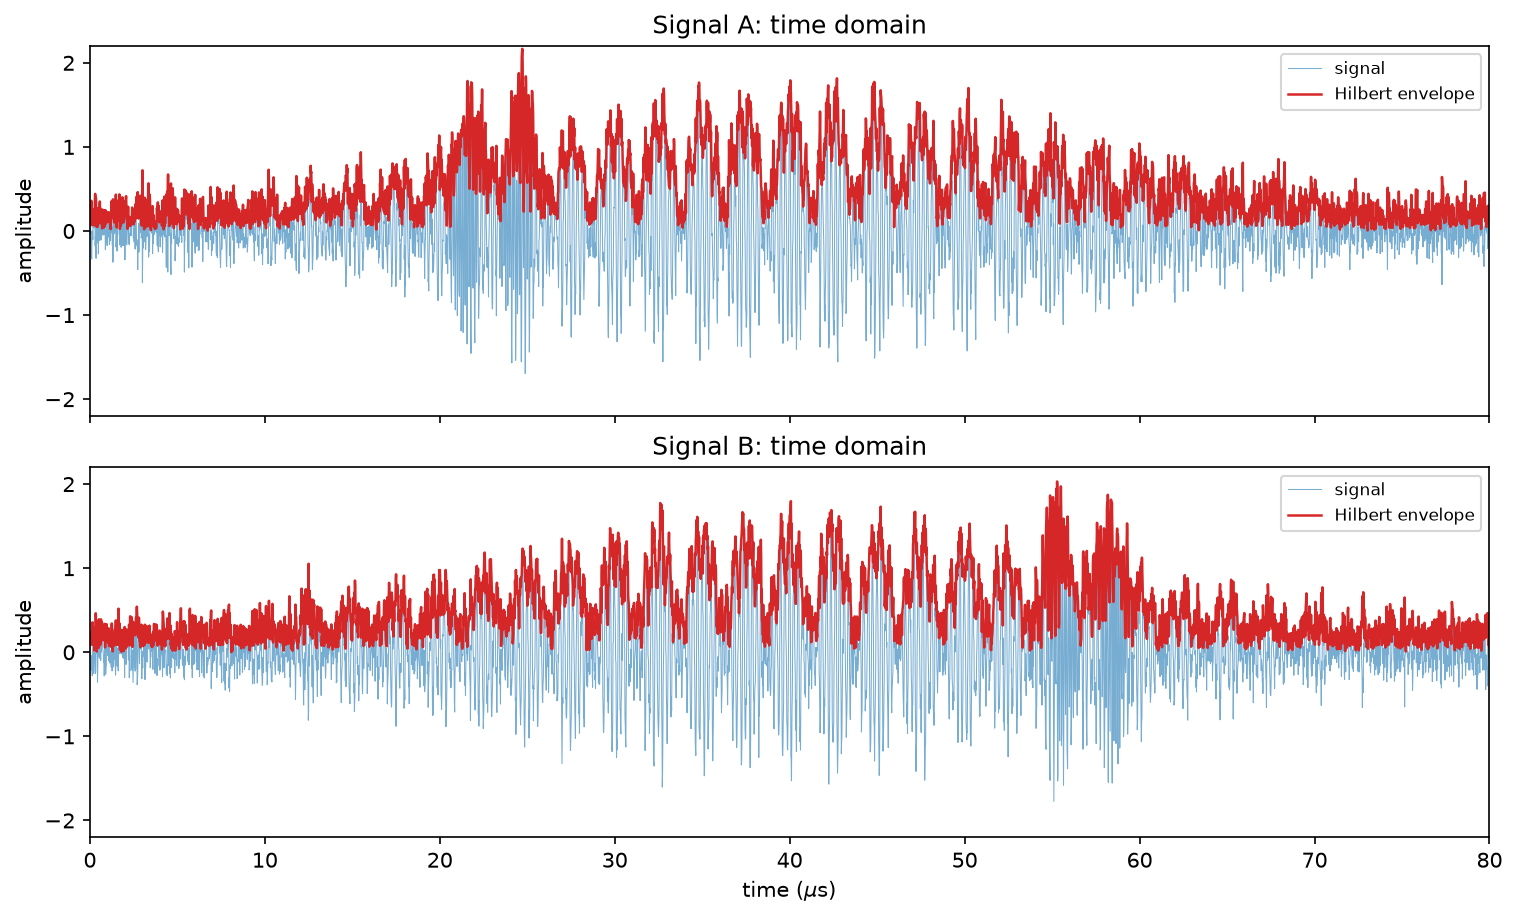
\includegraphics[width=\linewidth]{image/q1a_time_domain.png}
  \caption{Q1(a): time-domain waveforms with the Hilbert envelope overlaid
  (same limits for both panels). Signal A peaks early (envelope maximum at
  $24.7\us$); signal B peaks late ($55.3\us$). Both have nearly equal RMS
  amplitude ($0.472$ vs.\ $0.472$).}
  \label{fig:q1a}
\end{figure}

\begin{figure}[htbp]
  \centering
  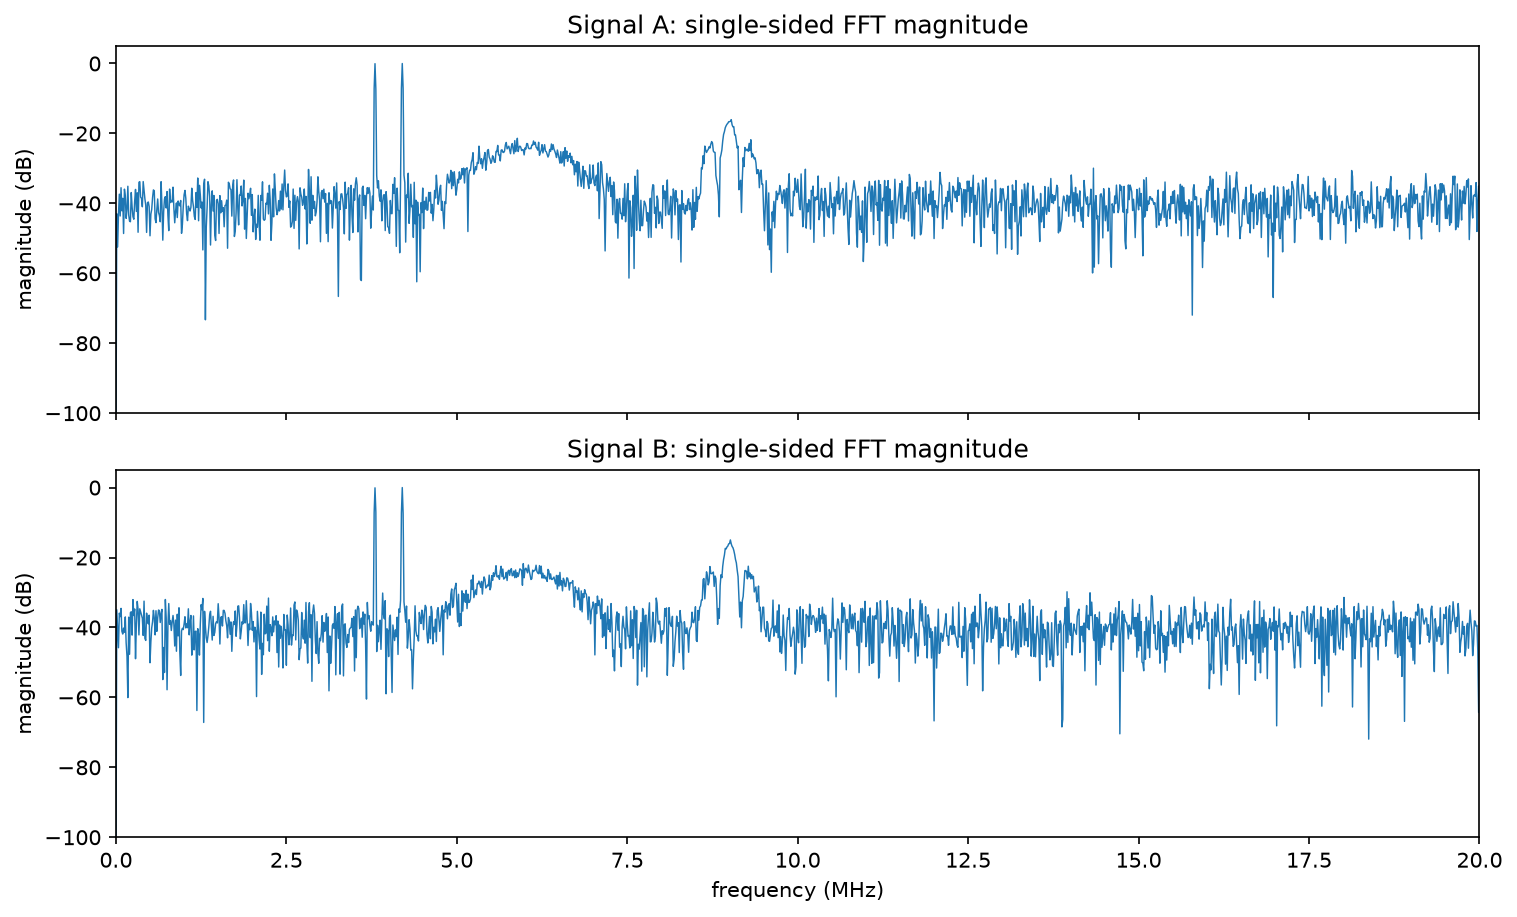
\includegraphics[width=0.95\linewidth]{image/q1a_fft_spectra.png}
  \caption{Q1(a): single-sided FFT magnitude, common normalization and common
  dB reference, identical axis limits. The two spectra are nearly
  indistinguishable.}
  \label{fig:q1afft}
\end{figure}

The time-domain signals look like band-limited noise bursts of almost identical
average power; only the envelope timing differs (A: $24.7\us$, B: $55.3\us$).
The FFT magnitude spectra are nearly identical: two sharp lines at
$3.800\MHz$ and $4.200\MHz$, a broad raised region from $\approx4.9$ to
$\approx7.1\MHz$, a line at $\approx9.0\MHz$, and an otherwise similar noise
floor.

The FFT magnitude alone cannot distinguish the temporal structures because it
is a time-averaged, phase-independent decomposition. Both recordings contain
the \emph{same} set of stationary spectral components, but arranged with
different time evolution. The magnitude spectrum discards the phase, so the
chirp direction, the chirp endpoints, and the arrival time of the 9\,\MHz
component are lost. In particular, the linear chirp spreads its energy over its
whole sweep, and its contribution and the fixed tones overlap in frequency,
which makes the spectral magnitudes of A and B look alike.

\subsection*{(b) STFT}

STFT parameters are exactly as required: Hann window of 240 samples
($4\us$), hop 6 samples ($0.1\us$), $N_{\mathrm{FFT}}=4096$, no detrending.
Boundary handling: \texttt{boundary=None} and \texttt{padded=False}, i.e.\ no
signal extension; only complete windows inside the record are used, so window
centers span $2$--$78\us$ and no padding or boundary extension is applied.
The two spectrograms
share one magnitude reference (the largest STFT magnitude of either signal) and
one color scale ($-80$ to $0$\,dB) (Fig.~\ref{fig:q1b}).

\begin{figure}[htbp]
  \centering
  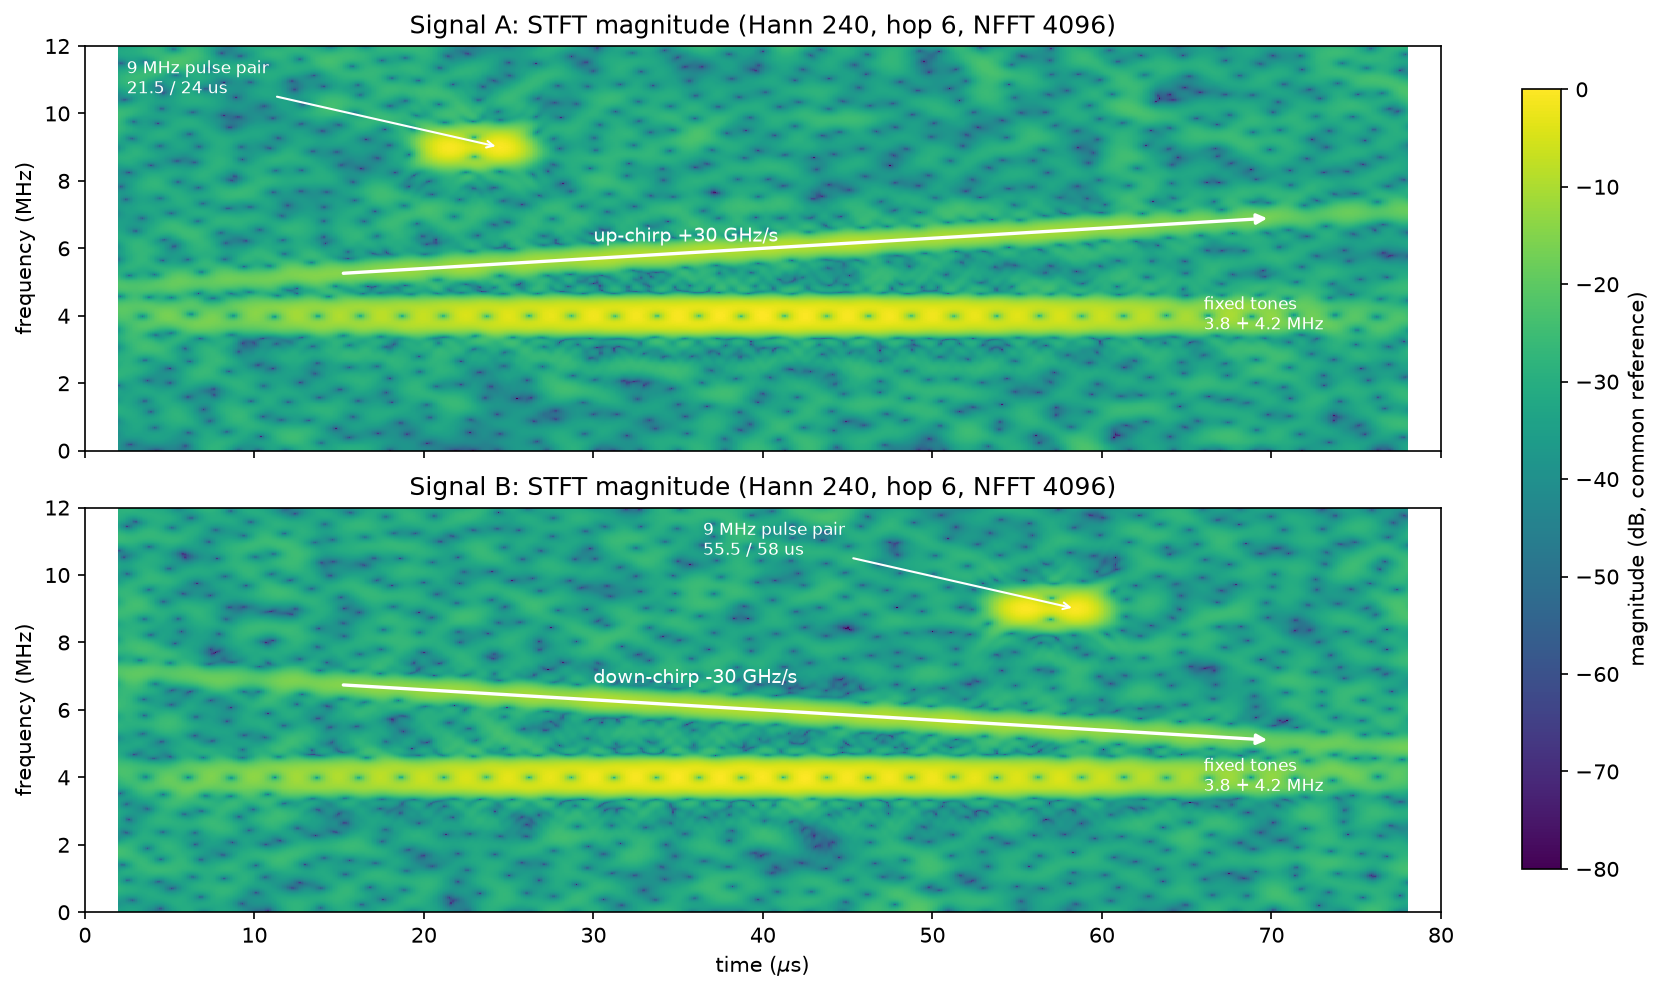
\includegraphics[width=\linewidth]{image/q1b_stft.png}
  \caption{Q1(b): required-parameter STFT of both signals, common
  normalization and color scale. The chirp direction and the pulse-pair time
  are the discriminating features.}
  \label{fig:q1b}
\end{figure}

The STFT reveals that the two signals are built from the same three
components placed differently in time:

\begin{enumerate}[leftmargin=1.4em]
  \item Two steady tones at $3.800\MHz$ and $4.200\MHz$ (separation
  $400$\,kHz), present over the whole record in both signals.
  \item A linear chirp. In A it sweeps \emph{up} from $\approx4.9\MHz$
  ($\approx4\us$) to $\approx7.1\MHz$ ($\approx76\us$), slope
  $\approx+30\GHz/s$; in B it sweeps \emph{down} from $\approx7.1\MHz$ to
  $\approx4.9\MHz$ with $\approx-30\GHz/s$.
  \item A narrowband component at $9.02\MHz$ (A) / $9.01\MHz$ (B) that appears
  as a \emph{pair} of short pulses: at $21.5\us$ and $24.5\us$ for A, and at
  $55.5\us$ and $58.5\us$ for B (lobe separation $2.97\us$, pulse widths
  $\approx1.7\us$ at $-6$\,dB).
\end{enumerate}

Thus the temporal order of the chirp and the timing of the 9\,MHz pulse pair
are the features that distinguish A from B, and they are directly visible in
the STFT as the opposite slope of the diagonal ridge and the different
locations of the 9\,MHz blobs.

\section{Question 2: STFT, CWT, and Time--Frequency Resolution}

\subsection*{(a) Short and long windows and the signal components}

Two representative windows were used, both with a Hann window, hop
$8$ samples ($0.133\us$), $N_{\mathrm{FFT}}=4096$, and no boundary extension:

\begin{itemize}[leftmargin=1.4em]
  \item \textbf{Short:} 128 samples ($2.13\us$). Hann main-lobe width
  $4f_s/N\approx1.88\MHz$. Gives good time localization.
  \item \textbf{Long:} 1024 samples ($17.07\us$). Hann main-lobe width
  $\approx0.234\MHz$. Gives good frequency localization.
\end{itemize}

Both spectrograms in Fig.~\ref{fig:q2a} use the same reference (largest
magnitude across the two) and the same $-80\ldots0$\,dB color scale.

\begin{figure}[htbp]
  \centering
  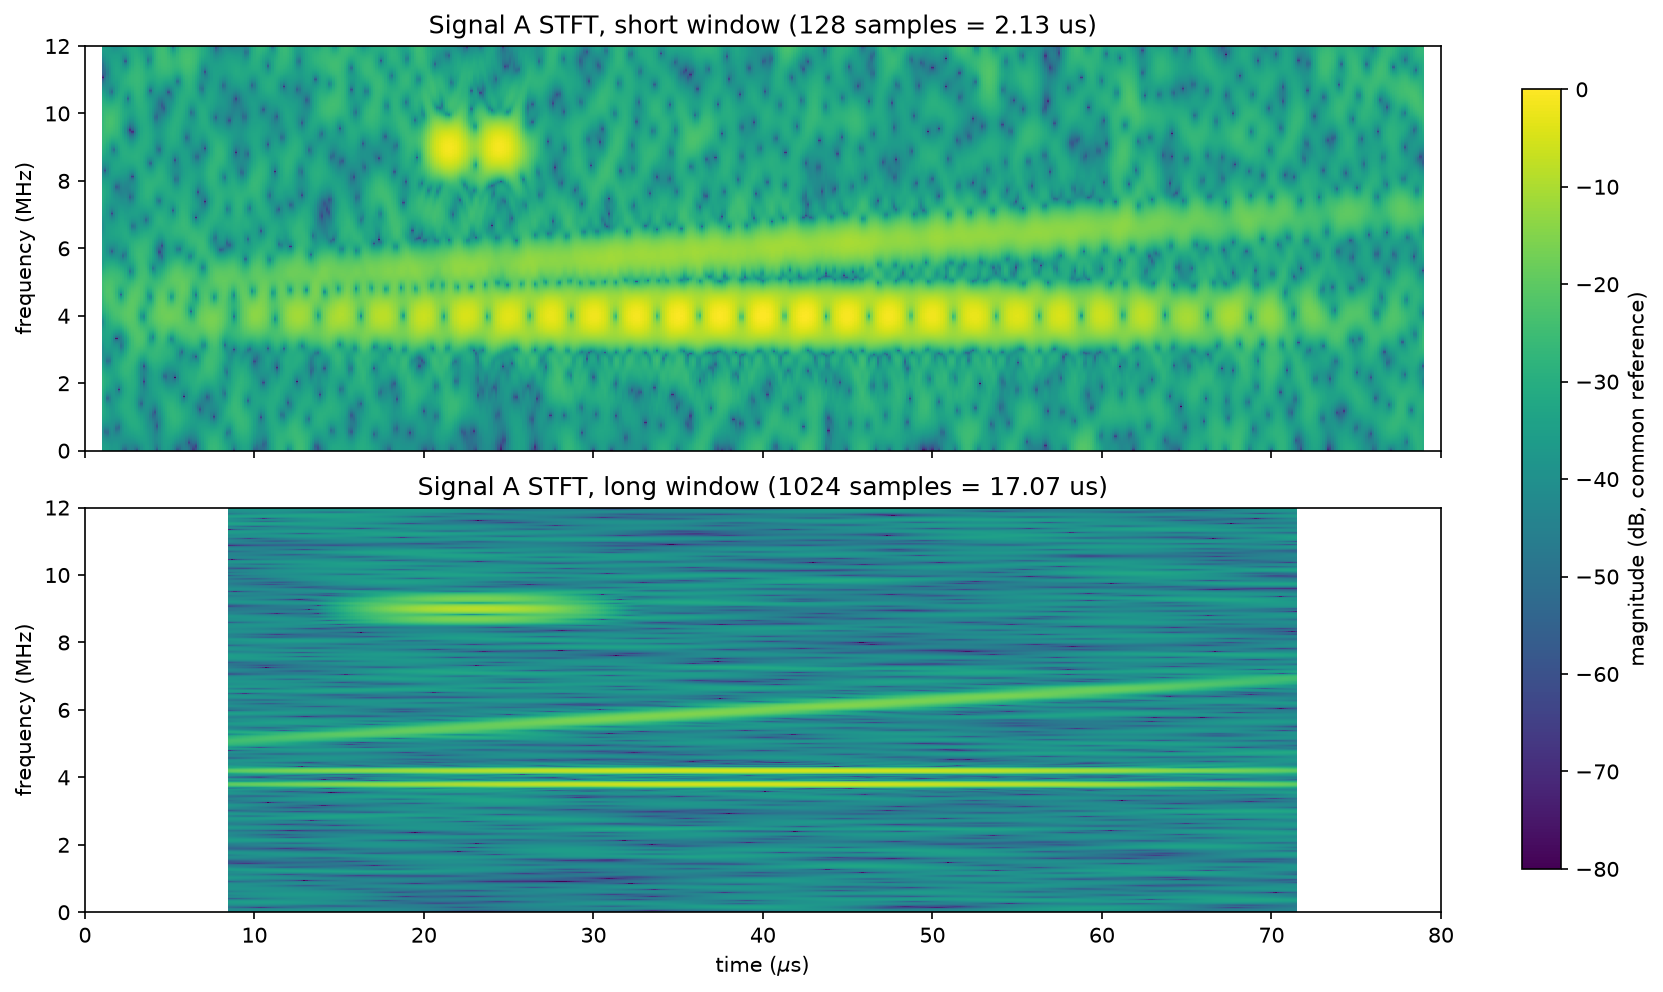
\includegraphics[width=\linewidth]{image/q2a_stft_windows.png}
  \caption{Q2(a): Signal A STFT with short and long windows, common
  normalization and color scale. The chirp is visible in both; the
  low-frequency tone doublet is only resolved by the long window.}
  \label{fig:q2a}
\end{figure}

\begin{figure}[htbp]
  \centering
  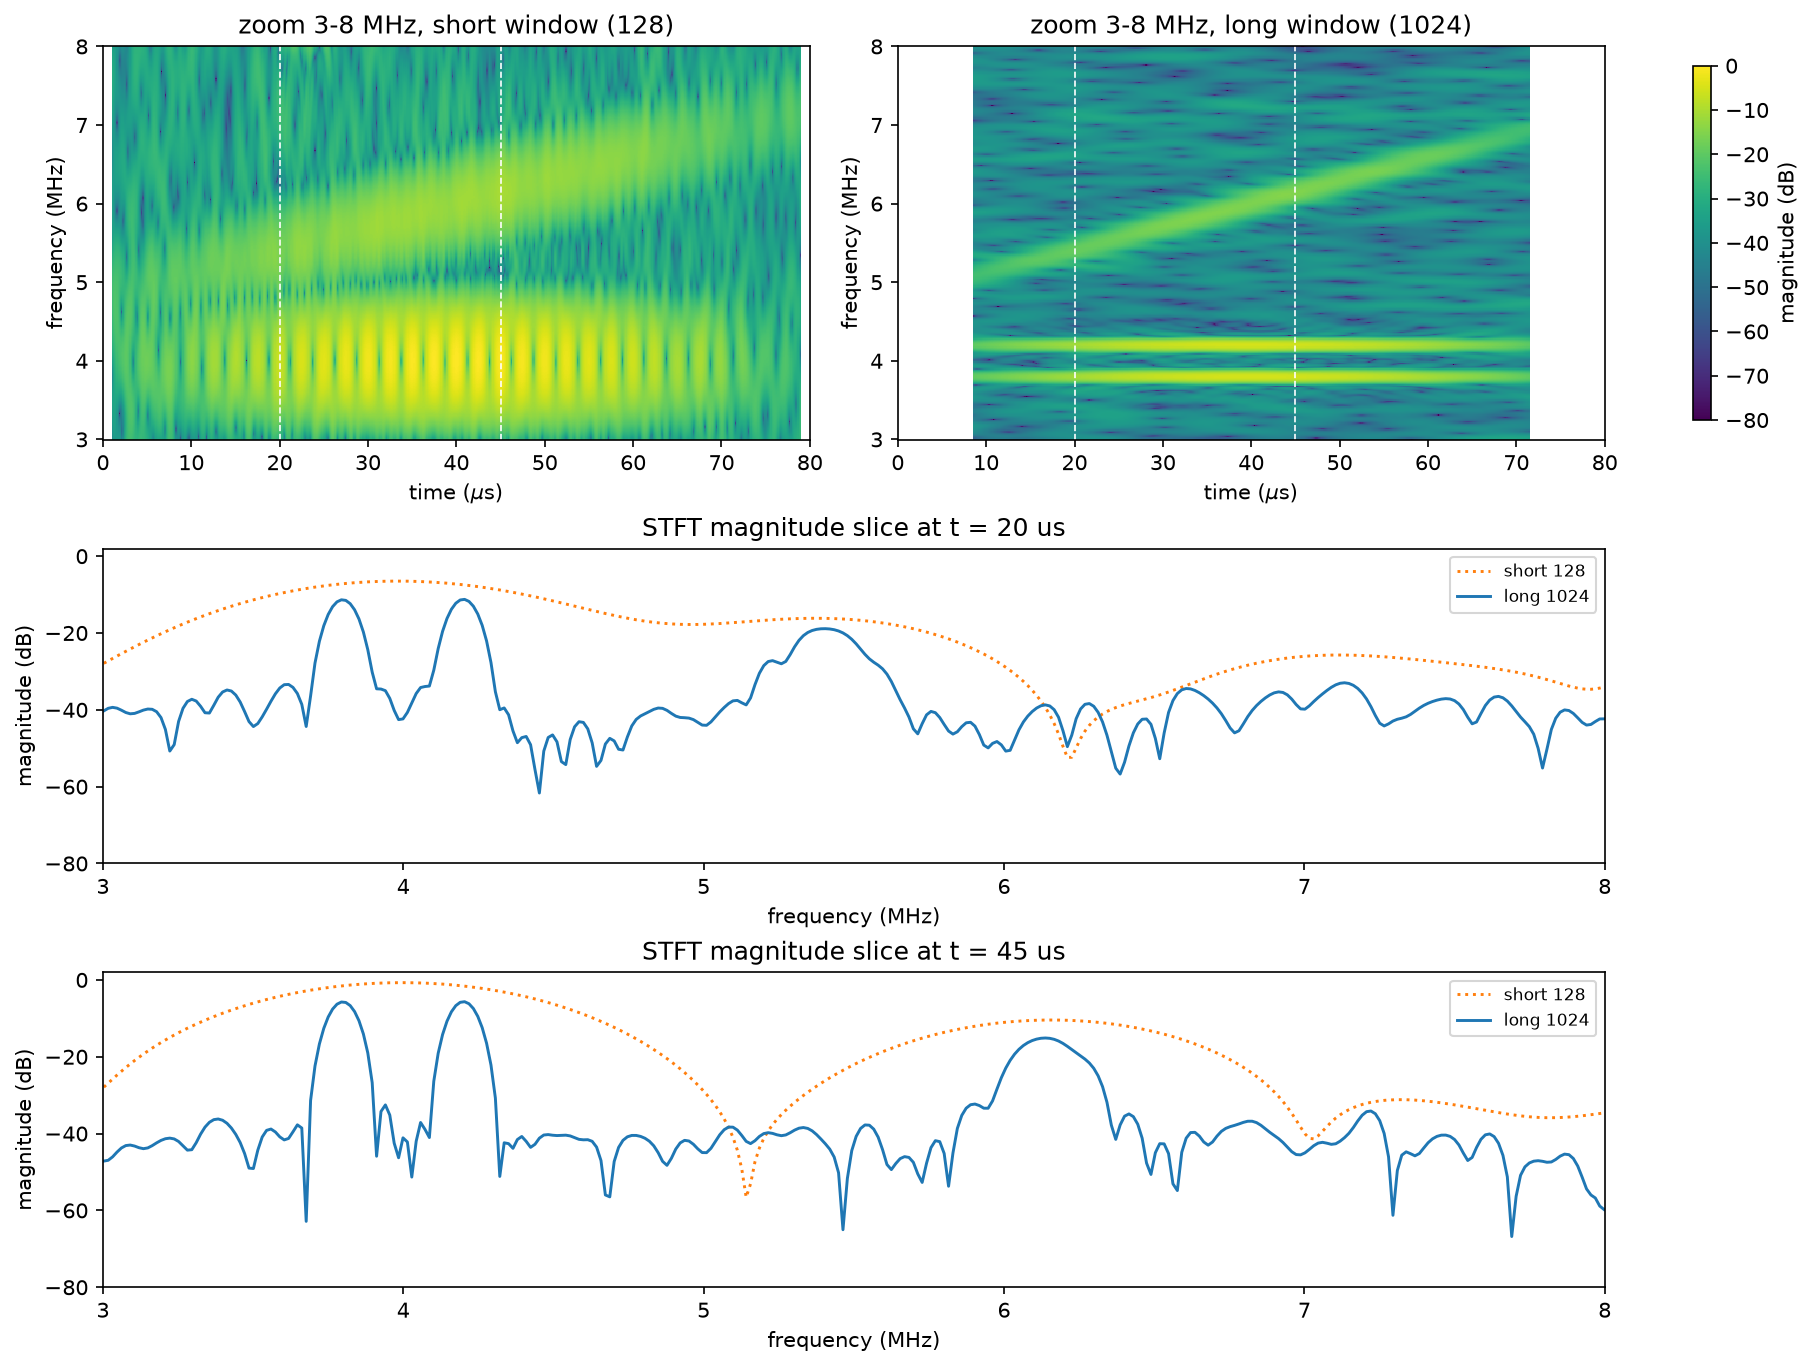
\includegraphics[width=\linewidth]{image/q2a_zoom_slices.png}
  \caption{Q2(a): 3--8\,MHz zooms (top) and 1-D STFT slices at 20 and $45\us$
  (bottom). The long window separates 3.800/4.200\,MHz and the chirp ridge;
  the short window merges them into one broad peak.}
  \label{fig:q2aslices}
\end{figure}

\textbf{Components of Signal A.}

\begin{enumerate}[leftmargin=1.4em]
  \item \textbf{Two steady tones} at $3.800\MHz$ and $4.200\MHz$, separation
  $0.400\MHz$, present for the full duration. The separation is obtained from
  the long-window spectrogram (and confirmed by the full-record FFT); the
  short-window main lobe ($1.88\MHz$) merges them into a single $4\MHz$ band.
  \item \textbf{Linear up-chirp} from $\approx4.9\MHz$ at $\approx4\us$ to
  $\approx7.1\MHz$ at $\approx76\us$. A line fit to the ridge (1024-sample
  window) gives $f(t)=4.84+0.0291\,t$ ($\MHz$, $\us$); a 512-sample window
  gives $4.80+0.0299\,t$. Both correspond to $+(29$--$30)\GHz/s$.
  The distance between the chirp and the upper tone grows with time:
  $0.78\MHz$ at $5\us$, $1.22\MHz$ at $20\us$, $1.95\MHz$ at $45\us$, and
  $2.82\MHz$ at $75\us$. The long window resolves the chirp from the tones at
  all these times; with the short window the chirp and the upper tone merge
  while their separation stays below its $1.88\MHz$ main lobe, i.e.\ before
  $\approx40\us$ (Fig.~\ref{fig:q2aslices}).
  \item \textbf{9\,MHz pulse pair} centered at $9.02\MHz$ with lobes at
  $21.5\us$ and $24.5\us$ (separation $2.97\us$, each lobe $\approx1.7\us$
  long at $-6$\,dB). The short window resolves the two lobes; the long window
  smears them into one blob (Fig.~\ref{fig:q2a}, lower panel).
\end{enumerate}

The slices in Fig.~\ref{fig:q2aslices} support these estimates directly: at
$t=20\us$ the long window shows three peaks (the tones at $3.8$ and
$4.2\MHz$ and the chirp at $\approx5.4\MHz$), while the short window shows one
broad peak; at $t=45\us$ the long window shows the tones and the chirp at
$\approx6.1\MHz$.

\subsection*{(b) Time--frequency resolution trade-off}

For a Hann window the time and frequency widths satisfy
$\Delta t\,\Delta f\approx4$ (samples$\cdot$bins): $\Delta t$ scales as $N/f_s$
while the main-lobe width scales as $4f_s/N$, so the product is fixed. For the
two windows used here:
\[
(2.13\us)(1.88\MHz)\approx4.0,\qquad
(17.07\us)(0.234\MHz)\approx4.0 .
\]
The short window (\ref{fig:q2a}, top) localizes each $1.7\us$ pulse and the
chirp endpoints in time, but merges the $0.400\MHz$ tone doublet and the
chirp with the tones at early times. The long window (bottom) separates the
tones and the chirp, but merges the two $9\MHz$ lobes and smears the chirp
onset/end by $\pm8.5\us$.

No single window resolves all components: resolving the $0.400\MHz$ doublet
requires a window of at least $\approx4f_s/0.4\MHz=600$ samples
($10\us$), which already merges the $3\us$-separated pulses; resolving the
pulse pair cleanly requires $\Delta t\lesssim1.5\us$ ($N\lesssim90$), which
merges the tones and the early chirp. The two estimates therefore need the two
spectrograms: frequencies and separations from the long window, times from the
short window.

\subsection*{(c) Continuous wavelet transform}

A complex Morlet wavelet \texttt{cmor1.5-1.0} (bandwidth $B=1.5$, center
frequency $C=1.0$ cycles/sample at scale 1) was used with 400 log-spaced
scales covering $2.5$--$12\MHz$ via $f=C f_s/a$. PyWavelets returns
$L_2$-normalized coefficients (unit-energy wavelet at each scale), whose
magnitude for a constant-amplitude tone grows as $\sqrt{a}$; each scale row was
therefore divided by $\sqrt{a}$ (per-scale $L_1$ normalization) so that
equal-amplitude components have comparable brightness. The dB display uses the
maximum compensated magnitude as reference, a $10^{-6}$ floor, and the
$-80\ldots0$\,dB scale (Fig.~\ref{fig:q2c}).

\begin{figure}[htbp]
  \centering
  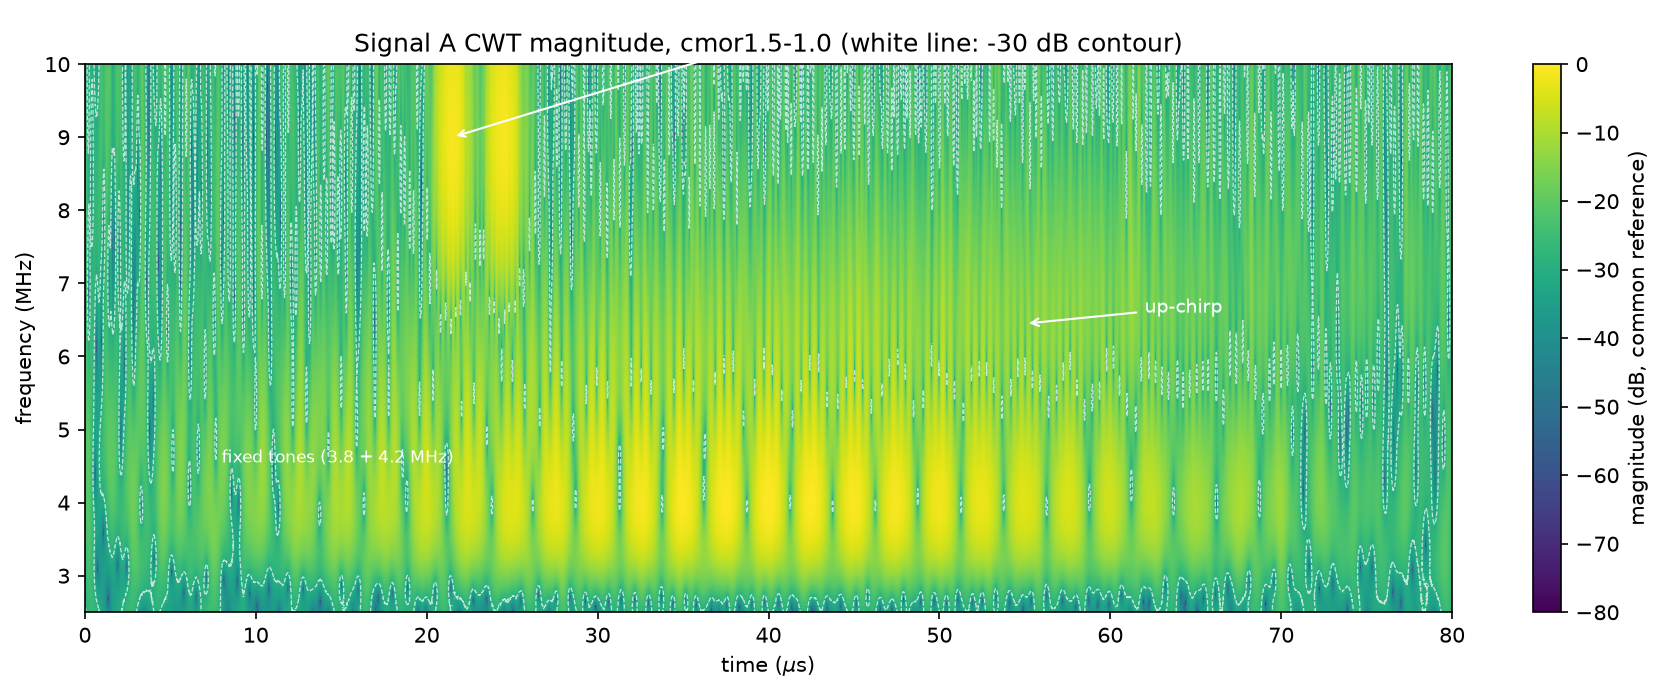
\includegraphics[width=\linewidth]{image/q2c_cwt.png}
  \caption{Q2(c): CWT magnitude of Signal A, \texttt{cmor1.5-1.0}
  (white line: $-30$\,dB contour). The wavelet adapts its resolution with
  frequency: it resolves the two $9\MHz$ pulses, tracks the chirp once it is
  separated from the tones, but merges the $400$\,kHz tone doublet.}
  \label{fig:q2c}
\end{figure}

\textbf{Comparison with the STFT.} The complex Morlet has a constant quality
factor $Q=f/\Delta f\approx2.7$. Its Gaussian bandwidth is therefore
$\approx1.5\MHz$ at $4\MHz$ and $\approx3.3\MHz$ at $9\MHz$, while its
effective time width is $\sigma_t\approx0.87/f$: $0.22\us$ at $4\MHz$ and
$0.10\us$ at $9\MHz$ (the product $\sigma_t\sigma_f$ is constant). The CWT
result shows:

\begin{itemize}[leftmargin=1.4em]
  \item the $9\MHz$ pulse pair is \emph{resolved} in time (two lobes), like the
  short STFT and unlike the long STFT;
  \item the chirp is visible once it separates from the tones
  ($f_{\text{chirp}}-f_{\text{tone}}\gtrsim Q$-limited bandwidth), i.e.\ after
  $\approx30$--$40\us$; at earlier times it merges with the tone band;
  \item the $3.800/4.200\MHz$ doublet is \emph{not} resolved, because its
  $0.4\MHz$ separation is far below the $1.5\MHz$ bandwidth at $4\MHz$; this is
  worse than the long STFT ($0.234\MHz$) and similar to the short STFT.
\end{itemize}

\textbf{Does the CWT eliminate the trade-off?} No. The CWT does not beat the
uncertainty relation; at each frequency it merely chooses a different point on
the $\Delta t$--$\Delta f$ hyperbola: long effective windows at low frequency
(good frequency resolution, coarse time) and short effective windows at high
frequency (good time resolution, coarse frequency). This is why it resolves
the high-frequency pulse pair but merges the low-frequency tone doublet at the
same time. Resolving the $0.400\MHz$ doublet at $4\MHz$ would require a
much higher-$Q$ analysis (e.g.\ a Morlet with large $B$, or the long STFT),
which in turn would smear the $3\us$-separated pulses. The evidence across
Figs.~\ref{fig:q2a}, \ref{fig:q2aslices} and \ref{fig:q2c} shows that the
limitation is fundamental, not a property of a particular transform.

\section{Question 3: Classifying Ultrasound Recordings}

Each recording has 896 samples at $f_s=26.5216\MHz$ ($33.8\us$). Features were
computed identically for the reference, Stage 1, and Stage 2 sets; no
per-recording normalization was applied.

\subsection*{Features and reference-set statistics}

The main feature is the amplitude envelope of the analytic signal
(Hilbert transform), smoothed by a centered five-point average. From it we
extract (all times in $\us$):

\begin{itemize}[leftmargin=1.4em]
  \item $a_{\text{main}}$: global envelope maximum;
  \item $a_{\text{early}}$, $t_{\text{early}}$: maximum envelope in
  $[5,22)\us$ and its time;
  \item $a_{\text{late}}$: maximum envelope for $t\ge22\us$;
  \item $\text{late\_ratio}=a_{\text{late}}/a_{\text{early}}$;
  \item $\text{doublet\_ratio}$: maximum envelope in
  $[t_{\text{early}}+2.1,\,t_{\text{early}}+3.4]\us$ divided by
  $a_{\text{early}}$, which detects a second surface echo $\approx2.75\us$
  after the main one.
\end{itemize}

\begin{table}[htbp]
  \centering
  \caption{Reference-set feature statistics (mean $\pm$ std, $n=15$ per class).}
  \begin{tabular}{lccc}
    \toprule
    Feature & Class 1 (acrylic) & Class 2 (sandpaper) & Class 3 (kitchen paper)\\
    \midrule
    $a_{\text{main}}$      & $1.072\pm0.112$ & $1.156\pm0.083$ & $0.519\pm0.064$\\
    $a_{\text{early}}$     & $1.072\pm0.112$ & $1.156\pm0.083$ & $0.282\pm0.118$\\
    $a_{\text{late}}$      & $0.061\pm0.011$ & $0.081\pm0.030$ & $0.478\pm0.138$\\
    late\_ratio            & $0.057\pm0.011$ & $0.069\pm0.023$ & $2.202\pm1.375$\\
    $t_{\text{early}}$ ($\us$) & $14.63\pm0.30$ & $12.40\pm0.12$ & $11.85\pm0.24$\\
    doublet\_ratio         & $0.319\pm0.041$ & $0.015\pm0.005$ & $0.014\pm0.009$\\
    \bottomrule
  \end{tabular}
  \label{tab:q3stats}
\end{table}

The classes have clear physical signatures (Figs.~\ref{fig:q3ref} and
\ref{fig:q3feat}):

\begin{itemize}[leftmargin=1.4em]
  \item \textbf{Class 1 (acrylic):} a strong echo at $\approx14.6\us$ followed
  by a strong secondary echo $2.75\us$ later (front and back surface of the
  plate), hence doublet\_ratio $0.20$--$0.39$.
  \item \textbf{Class 2 (sandpaper):} one dominant echo at $\approx12.4\us$
  with no nearby secondary echo (doublet\_ratio $\le0.023$) and only weak late
  scattering ($a_{\text{late}}\le0.17$).
  \item \textbf{Class 3 (kitchen paper):} weak echoes overall
  ($a_{\text{main}}<0.63$): an early echo at $\approx12\us$ and a later weak
  echo at $\approx26.5\us$ (late\_ratio up to $\approx5$). Within-class
  variation is larger here: in one recording (REF037) the late echo is almost
  absent, and in two recordings (REF031, REF037) the early echo is stronger
  than the late one.
\end{itemize}

\begin{figure}[htbp]
  \centering
  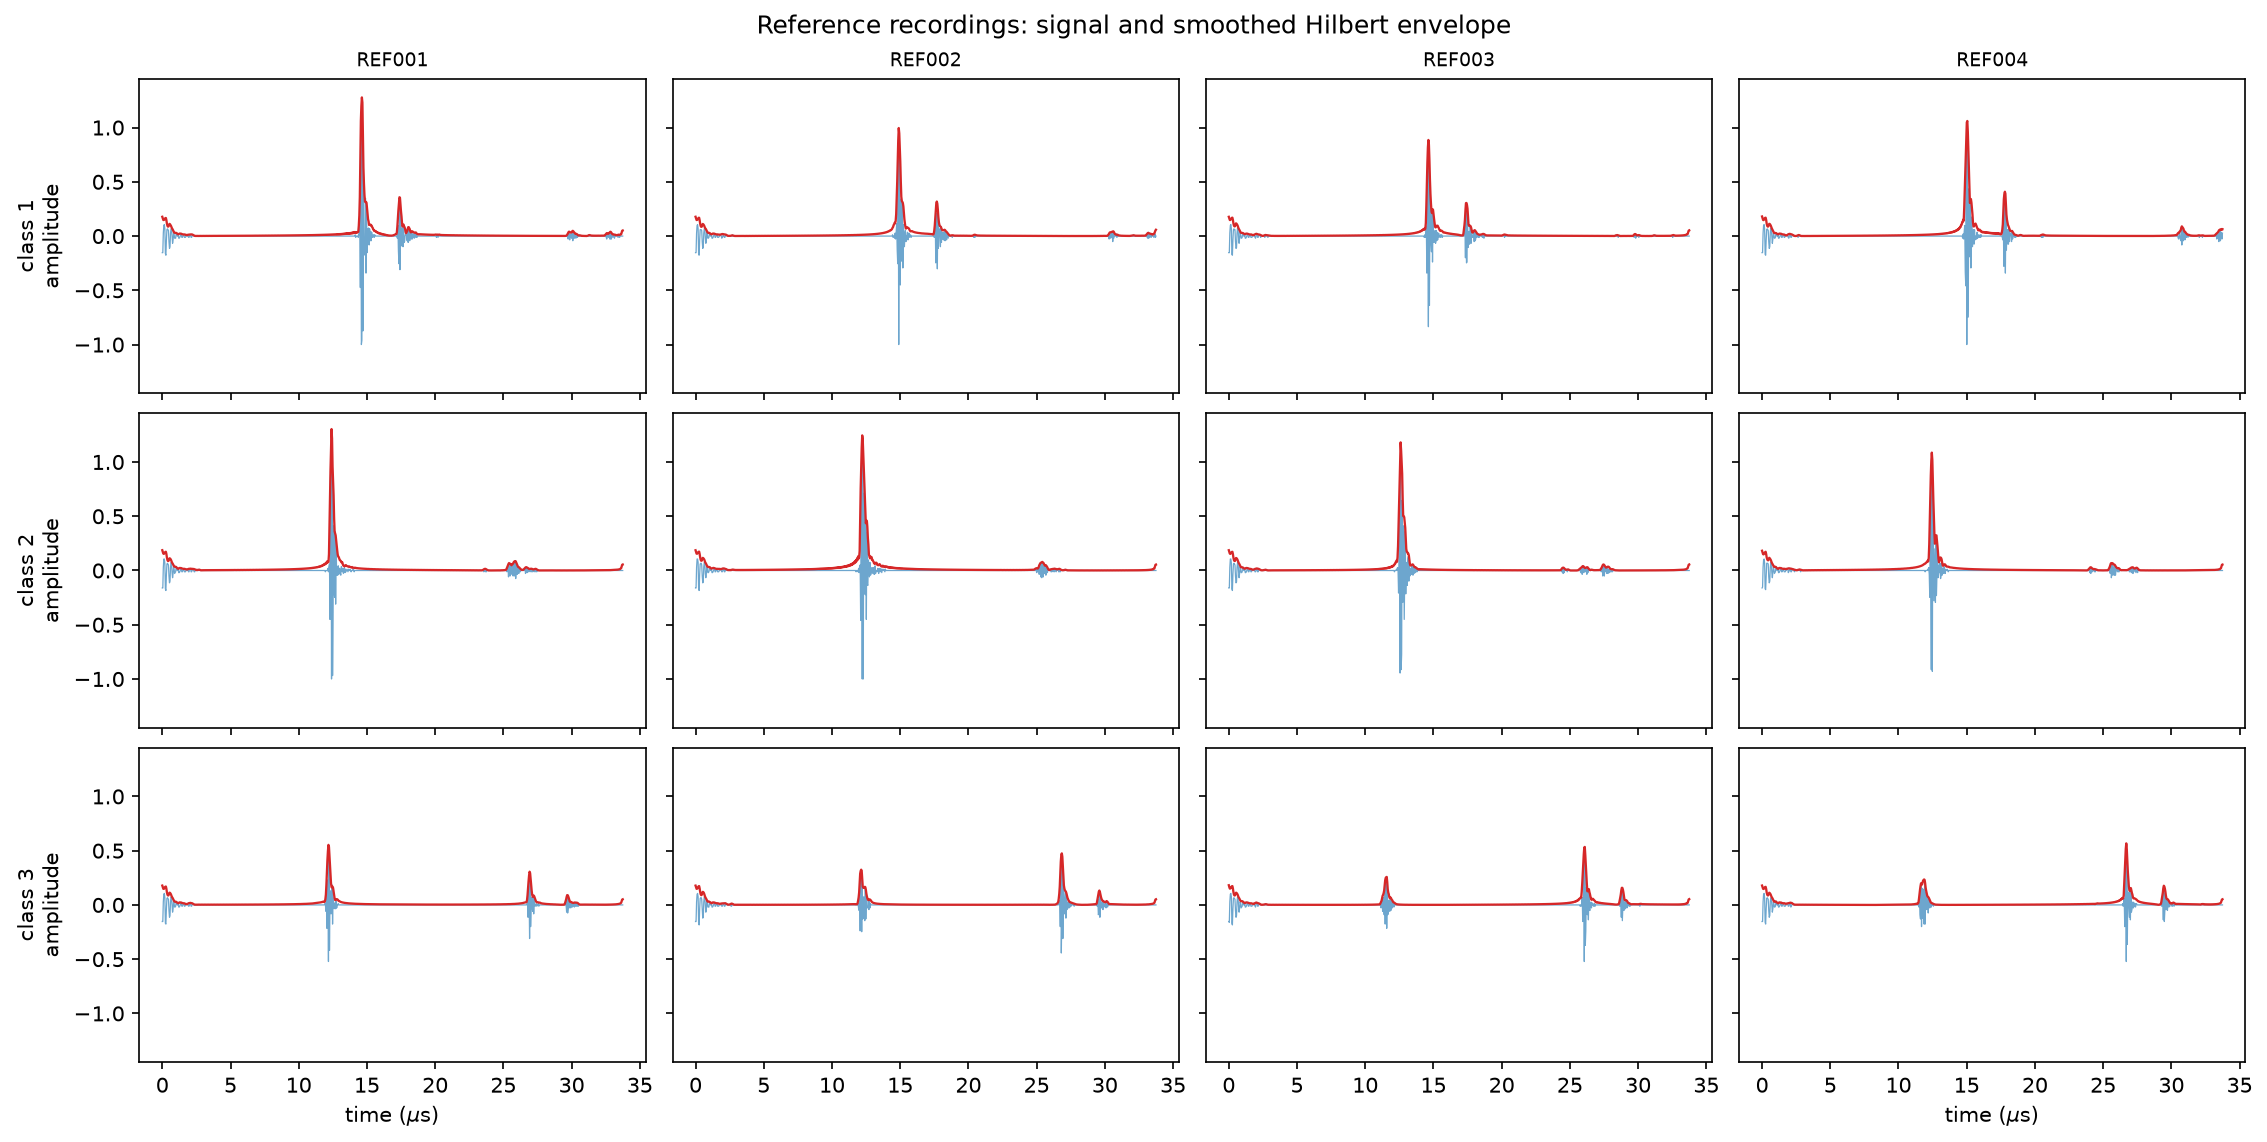
\includegraphics[width=\linewidth]{image/q3_reference_signals.png}
  \caption{Q3: four reference recordings per class (blue: signal, red:
  smoothed Hilbert envelope). Class 1 shows a double echo; class 2 a single
  strong echo; class 3 weak early/late echoes.}
  \label{fig:q3ref}
\end{figure}

\begin{figure}[htbp]
  \centering
  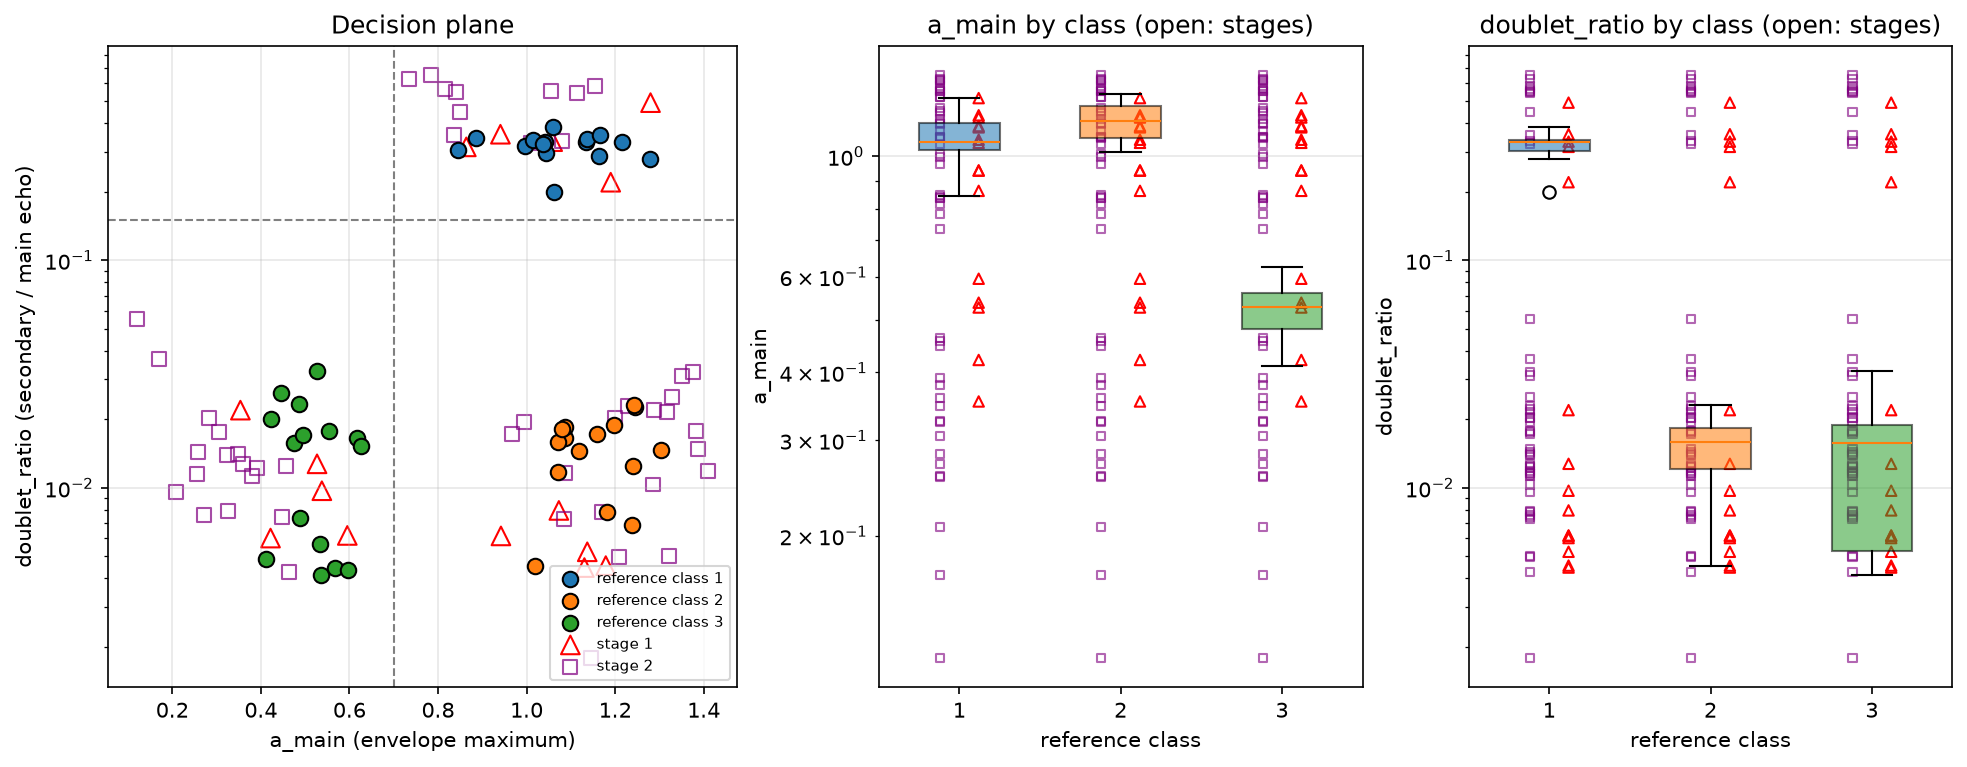
\includegraphics[width=\linewidth]{image/q3_features.png}
  \caption{Q3: decision plane (left) with the two thresholds, and class-wise
  distributions of $a_{\text{main}}$ and doublet\_ratio including the Stage 1
  (triangles) and Stage 2 (squares) recordings.}
  \label{fig:q3feat}
\end{figure}

\begin{figure}[htbp]
  \centering
  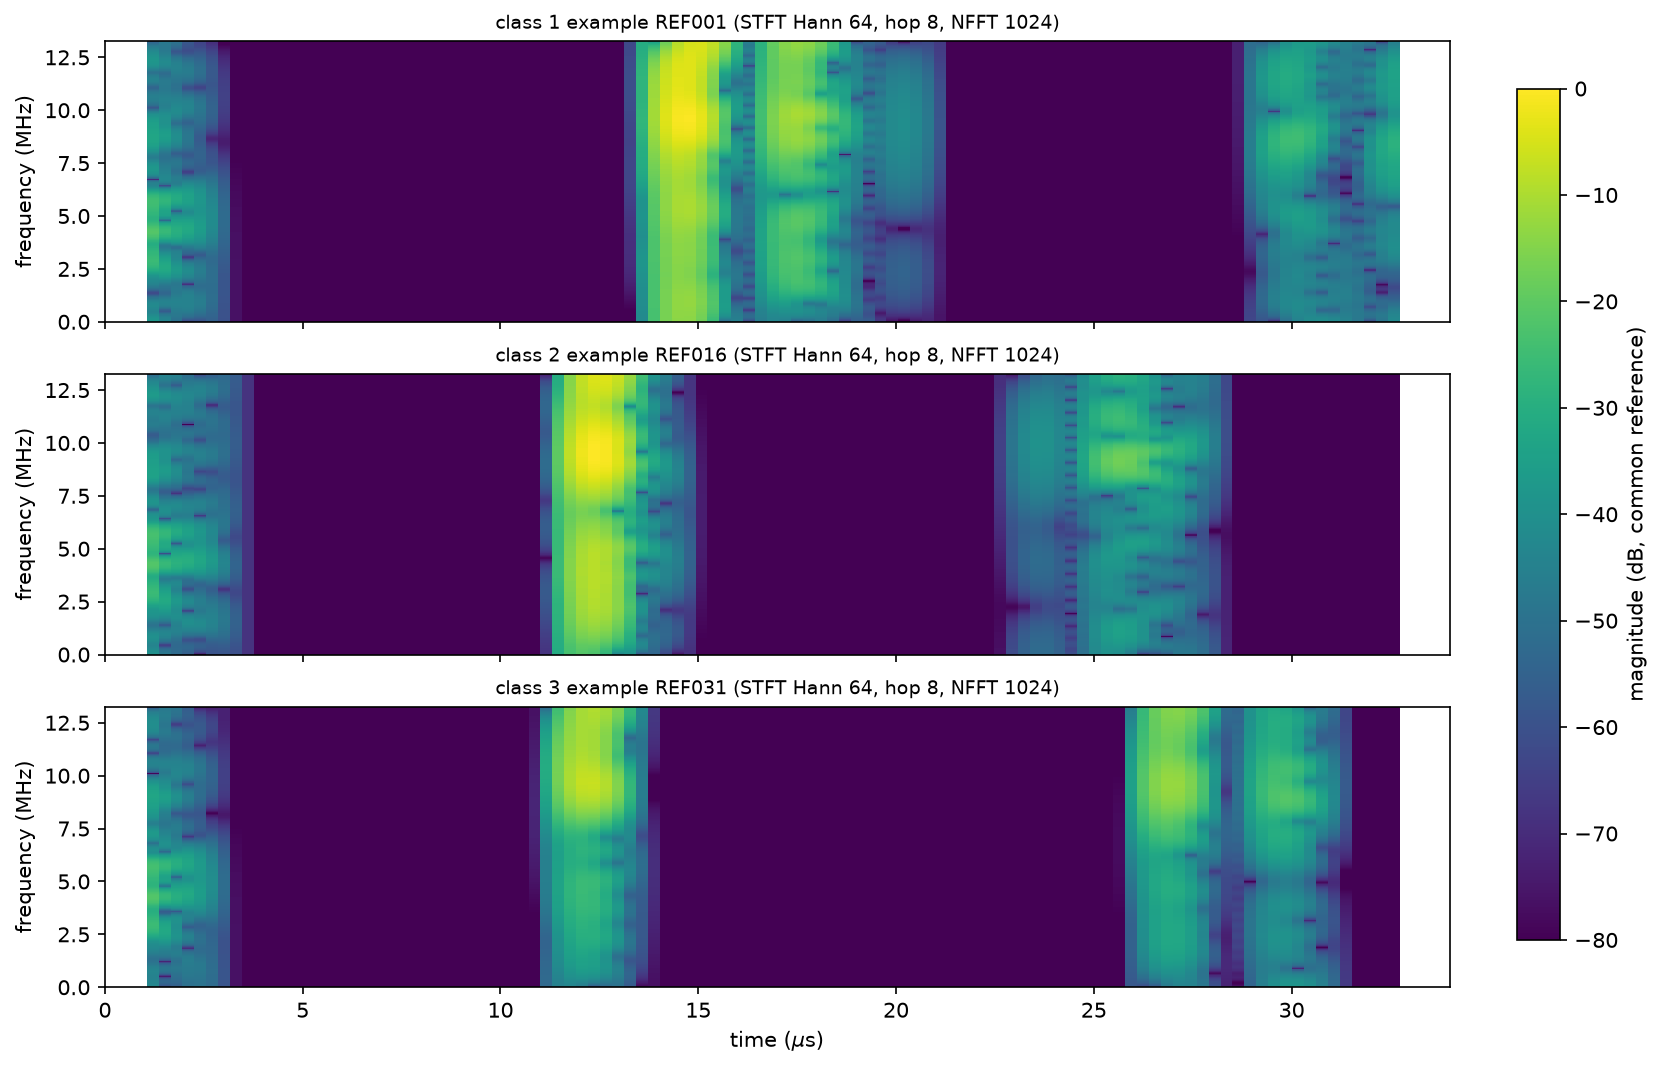
\includegraphics[width=\linewidth]{image/q3_stft_examples.png}
  \caption{Q3: example STFT magnitude (Hann 64, hop 8, NFFT 1024) of one
  reference recording per class, common normalization and color scale
  (dB convention as required).}
  \label{fig:q3stft}
\end{figure}

\subsection*{Decision rules}

The thresholds below were chosen from the labeled reference set only, using
the visible gaps in Fig.~\ref{fig:q3feat}:

\begin{enumerate}[leftmargin=1.4em]
  \item \textbf{If doublet\_ratio $>0.15$: class 1.}
  Reference margin: class 1 minimum $0.201$ vs.\ maximum $0.033$ for classes
  2 and 3.
  \item \textbf{Else if $a_{\text{main}}<0.70$: class 3.}
  Reference margin: class 3 maximum $0.626$ vs.\ minimum $0.845$ for classes
  1 and 2.
  \item \textbf{Otherwise: class 2.}
\end{enumerate}

These explicit rules classify all 45 labeled reference recordings correctly
(45/45, 100\%). As an optional cross-check, a linear discriminant analysis on
$[a_{\text{main}},\text{late\_ratio},\text{doublet\_ratio}]$ with
leave-one-out evaluation also reaches 100\%. The rules use ratios and echo
timing, which are more robust to the handling differences of the classroom
recordings than absolute amplitudes: in Stage 2 the strongest-echo time ranges
from $10.3$ to $16.1\us$, while the doublet pattern stays stable.

\subsection*{Task-stage predictions}

Applying the same frozen rules to the anonymized sets (Eq.~above; no labels
used):

\begin{itemize}[leftmargin=1.4em]
  \item \textbf{Stage 1} (\texttt{predictions\_stage1.csv}, 15 recordings):
  5 class 1, 5 class 2, 5 class 3. All 15 fall far from the thresholds, and
  the 5-per-class counts expected for this TA-collected set are reproduced.
  \item \textbf{Stage 2} (\texttt{predictions.csv}, 47 recordings):
  11 class 1, 19 class 2, 17 class 3.
\end{itemize}

The class-3 group in Stage 2 includes both weak-echo patterns seen in the
reference set (strong-late-echo and weak-early-echo-only), which is the main
within-class variation observed. We do not report accuracy against the
withheld labels, as required.

\end{document}
